\documentclass{article}
\usepackage[utf8]{inputenc}
\usepackage[english]{babel}
\usepackage[]{amsthm} %lets us use \begin{proof}
\usepackage[]{amssymb} %gives us the character \varnothing
\usepackage[]{setspace} %provides commands to set line spacing
\usepackage[left=0.75in, right=0.75in]{geometry}
\usepackage{hyperref}
\usepackage{xcolor}
\usepackage{amsmath}
\usepackage{enumitem}
\usepackage{graphicx}
\usepackage{subfigure}
\usepackage{float}
\title{Homework 2}
\author{Son [Joe] Nguyen}
%\date{\today}

\begin{document}
%\maketitle %This command prints the title based on information entered above
\begin{center}
	\LARGE{Homework 3}\\[1em]
	\large Son [Joe] Nguyen\\[1em]
	%\large \today
\end{center}
\subsection*{Problem 2.10}
From equation 2.60 in the text book, we have:
\[\psi_0(x) = \left(\frac{m \omega}{\pi \hbar}\right)^\frac{1}{4} e^{-\frac{m \omega}{2\hbar}x^2}\]

\noindent From equation 2.48, we have:
\[\hat{a}_\pm \equiv \frac{1}{\sqrt{2 \hbar m \omega}} \left(\mp i\hat{p} + m \omega x\right)\]

\noindent And the formula for $\psi_n(x)$ is:
\[\psi_n = \frac{1}{\sqrt{n!}} \left(\hat{a}_+\right)^n \psi_0\]

\noindent Therefore we have \(\psi_2(x) = \frac{1}{\sqrt{2!}} (\hat{a}_+)^2 \psi_0\)
\\
\\
\noindent We can calculate \((\hat{a}_+)^2 \psi_0\) as follows:
\begin{align*}
	\hat{a}_+\psi_0                 & = \frac{1}{\sqrt{2 \hbar m \omega}} \left(\hbar \frac{d}{dx} + m \omega x\right) \left(\frac{m \omega}{\pi \hbar}\right)^{\frac{1}{4}} e^{-\frac{m \omega}{2\hbar}x^2}\quad \text{where } \hat{p} = -i\hbar \frac{d}{dx}         \\
	                                & = \frac{1}{\sqrt{2 \hbar m \omega}} \left(\frac{m \omega}{\pi \hbar}\right)^{\frac{1}{4}} \left[\hbar \frac{d}{dx} \left(e^{-\frac{m \omega}{2\hbar}x^2}\right) + m \omega x \left(e^{-\frac{m \omega}{2\hbar}x^2}\right)\right] \\
	                                & = \frac{1}{\sqrt{2 \hbar m \omega}} \left(\frac{m \omega}{\pi \hbar}\right)^{\frac{1}{4}} \left[2m\omega x \left(e^{-\frac{m \omega}{2\hbar}x^2}\right)\right]                                                                   \\
	\left(\hat{a}_+\right)^2 \psi_0 & = \frac{2 m \omega}{2 \hbar m \omega} \left(\frac{m \omega}{\pi \hbar}\right)^{\frac{1}{4}} \left(- \hbar \frac{d}{dx} + m \omega x \right) \left(x e^{-\frac{m \omega}{2\hbar}x^2} \right)                                      \\
	                                & = \frac{1}{\hbar} \left(\frac{m \omega}{\pi \hbar}\right)^{\frac{1}{4}} \left(- \hbar \frac{d}{dx} x e^{-\frac{m \omega}{2\hbar}x^2} + m \omega x^2 e^{-\frac{m \omega}{2\hbar}x^2} \right)                                      \\
	                                & = \frac{1}{\hbar} \left(\frac{m \omega}{\pi \hbar}\right)^{\frac{1}{4}} \left(-\hbar e^{-\frac{m \omega}{2\hbar}x^2} + 2 m \omega x^2 e^{-\frac{m \omega}{2\hbar}x^2}\right)
\end{align*}
So \(\psi_2(x) = \frac{1}{\sqrt{2}} \frac{1}{\hbar} \left(\frac{m \omega}{\pi \hbar}\right)^{\frac{1}{4}} \left(-\hbar e^{-\frac{m \omega}{2\hbar}x^2} + 2 m \omega x^2 e^{-\frac{m \omega}{2\hbar}x^2}\right) \)


\begin{figure}[H]
	\centering
	\subfigure[Plot of \(\psi_0(x)\)]{
		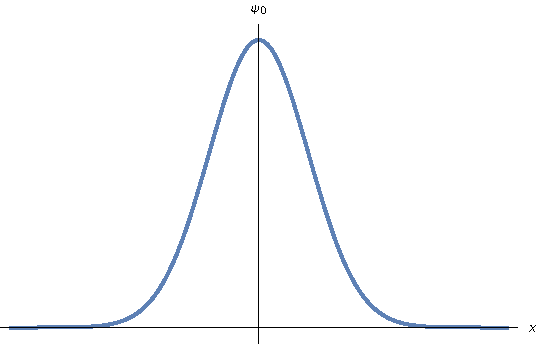
\includegraphics[width=0.3\linewidth]{Psi_0.pdf}
		\label{fig:psi_0}
	}
	\subfigure[Plot of \(\psi_1(x)\)]{
		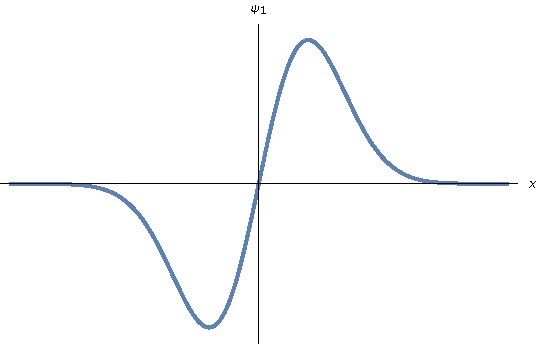
\includegraphics[width=0.3\linewidth]{Psi_1.pdf}
		\label{fig:psi_1}
	}
	\subfigure[Plot of \(\psi_2(x)\)]{
		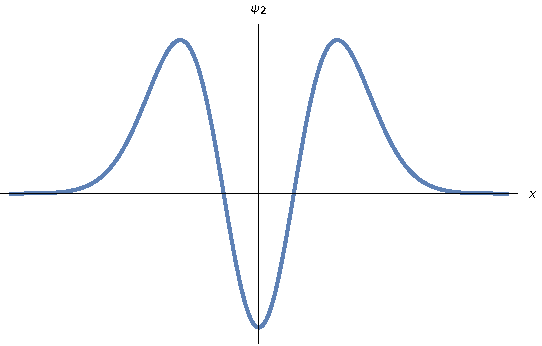
\includegraphics[width=0.3\linewidth]{Psi_2.pdf}
		\label{fig:psi_2}
	}
	\caption{Plots of \(\psi_n(x)\) for \(n=0, 1, 2\)}
\end{figure}


\noindent To check the orthogonality of the wave functions, we can calculate the integral of the product of the wave functions over the range of \([- \infty, \infty]\). If the integral is zero, then the wave functions are orthogonal. As we can see from the sketch. We have \(\psi_0(x)\) is an even function, \(\psi_1(x)\) is an odd function, and \(\psi_2(x)\) is an even function. Therefore, the product of \(\psi_0(x)\) and \(\psi_1(x)\) is an odd function, and the product of \(\psi_1(x)\) and \(\psi_2(x)\) is also an odd function.
So the integral of the product of \(\psi_0(x)\) and \(\psi_1(x)\) over the range of \([- \infty, \infty]\) is zero, and the integral of the product of \(\psi_1(x)\) and \(\psi_2(x)\) over the range of \([- \infty, \infty]\) is also zero. Therefore, the wave functions are orthogonal.
\begin{align*}
	\int_{-\infty}^{\infty} \psi_0(x) \psi_2(x) dx & = \int_{-\infty}^{\infty} \left(\frac{m \omega}{\pi \hbar}\right)^{\frac{1}{4}} e^{-\frac{m \omega}{2\hbar}x^2} \frac{1}{\sqrt{2}} \frac{1}{\hbar} \left(\frac{m \omega}{\pi \hbar}\right)^{\frac{1}{4}} \left(-\hbar e^{-\frac{m \omega}{2\hbar}x^2} + 2 m \omega x^2 e^{-\frac{m \omega}{2\hbar}x^2}\right) dx \\
	                                               & = \int_{-\infty}^{\infty} \left(\frac{m \omega}{\pi \hbar}\right)^{\frac{1}{4}} e^{-\frac{m \omega}{2\hbar}x^2} \frac{1}{\sqrt{2}} \left(\frac{m \omega}{\pi \hbar}\right)^{\frac{1}{4}} \left(\frac{2 m \omega x^2}{\hbar} -1 \right) e^{-\frac{m \omega}{2\hbar}x^2} dx = 0                                    \\
\end{align*}
\subsection*{Problem 2.11}
\[\psi_0(x) = \left(\frac{m \omega}{\pi \hbar}\right)^\frac{1}{4} e^{-\frac{m \omega}{2\hbar}x^2}\]

Set constant \(A = \left(\frac{m \omega}{\pi \hbar}\right)^\frac{1}{4}\), we have:
\[\psi_0(x) = A e^{-\frac{m \omega}{2\hbar}x^2}\]

\begin{align*}
	\langle x \rangle & = \int_{-\infty}^{\infty} x |\psi_0(x)|^2 dx                             \\
	                  & = \int_{-\infty}^{\infty} x (A e^{-\frac{m \omega}{2\hbar}x^2})^2 dx = 0 \\
\end{align*}

We have \(\langle p \rangle = m \frac{d \langle x \rangle }{dt} = 0 \), because \(\langle x \rangle = 0\). Therefore, the expectation value of the momentum is zero.
\\
\begin{align*}
	\langle x^2 \rangle & = \int_{-\infty}^{\infty} x^2 |\psi_0(x)|^2 dx                                                   \\
	                    & = \int_{-\infty}^{\infty} x^2 (A e^{-\frac{m \omega}{2\hbar}x^2})^2 dx = \frac{\hbar}{2m \omega} \\
\end{align*}

\[\langle p^2 \rangle = \int_{-\infty}^{\infty} \Psi(x,t)^* \left(\frac{\hbar}{i} \frac{d}{dx}\right)^2 \Psi(x,t)dx\]

\begin{align*}
	\langle p^2 \rangle & = \int_{-\infty}^{\infty} \psi_0(x) \left(\frac{\hbar}{i} \frac{d}{dx}\right)^2 \psi_0(x) dx                                                                                                          \\
	                    & = \int_{-\infty}^{\infty} (A e^{-\frac{m \omega}{2\hbar}x^2}) \left(\frac{\hbar}{i} \frac{d}{dx}\right)^2 (A e^{-\frac{m \omega}{2\hbar}x^2}) dx                                                      \\
	                    & = -\hbar^2 \int_{-\infty}^{\infty} A e^{-\frac{m \omega}{2\hbar}x^2} \frac{d^2}{dx^2} (A e^{-\frac{m \omega}{2\hbar}x^2}) dx                                                                          \\
	                    & = -\hbar^2 \int_{-\infty}^{\infty} A e^{-\frac{m \omega}{2\hbar}x^2} A \left(-\frac{e^{\frac{-m \omega x^2}{2\hbar}}}{h} + \frac{e^{\frac{-m \omega x^2}{2\hbar}}m^2 \omega^2 x^2}{\hbar^2}\right) dx \\
	                    & = \frac{m \omega \hbar}{2}
\end{align*}
\noindent We have the equation of \(\psi_1(x) = \left(\frac{m \omega}{\pi \hbar}\right)^{\frac{1}{4}} \sqrt{\frac{2m\omega}{\hbar}}xe^{\frac{m\omega}{2\hbar}x^2}\)
\begin{align*}
	\langle x \rangle & = \int_{-\infty}^{\infty} x |\psi_1(x)|^2 dx                                                                                                                        \\
	                  & = \int_{-\infty}^{\infty} x \left(\left(\frac{m \omega}{\pi \hbar}\right)^{\frac{1}{4}} \sqrt{\frac{2m\omega}{\hbar}}xe^{\frac{m\omega}{2\hbar}x^2}\right)^2 dx = 0 \\
\end{align*}
Therefore, \(\langle p \rangle = 0\)
\begin{align*}
	\langle x^2 \rangle & = \int_{-\infty}^{\infty} x^2 |\psi_1(x)|^2 dx \quad \text{set \(\alpha = \left(\frac{m \omega}{\pi \hbar}\right)^{\frac{1}{4}}\) and \(\beta = \sqrt{\frac{m\omega}{\hbar}x}\)}                  \\
	                    & = \int_{-\infty}^{\infty} x^2 \left(\alpha \sqrt{2}\beta e^{\frac{-y^2}{2}}\right)^2dx                                                                                                            \\
	                    & = \int_{-\infty}^{\infty} \frac{\hbar}{m \omega} \beta^2 (2\alpha^2 \beta^2 e^{-y^2}) \sqrt{\frac{\hbar}{m \omega}} d\beta                                                                        \\
	                    & =  \frac{3 \alpha^2 \hbar^2 \sqrt{\pi}}{2m^2 \sqrt{\frac{h \omega}{m}}}                                                                                                                           \\
	\langle p^2 \rangle & = \int_{-\infty}^{\infty} \psi_1(x) \left(\frac{\hbar}{i} \frac{d}{dx}\right)^2 \psi_1(x) dx                                                                                                      \\
	                    & = -\hbar^2 \int_{-\infty}^{\infty} \psi_1(x) \frac{d^2 \psi_1(x)}{dx^2} dx                                                                                                                        \\
	                    & = -\hbar^2 \int_{-\infty}^{\infty} \left(\alpha \sqrt{2}\beta e^{\frac{-y^2}{2}}\right) \frac{d^2}{dx^2} \left(\alpha \sqrt{2}\beta e^{\frac{-y^2}{2}}\right) \sqrt{\frac{\hbar}{m \omega}}d\beta \\
	                    & = -\hbar^2 \int_{-\infty}^{\infty} \sqrt{2} \alpha \beta e^{\frac{-y^2}{2}} \left(\sqrt{2} \alpha \frac{m \omega}{\hbar} (-3y + y^3)e^{\frac{-y^2}{2}}\right)\sqrt{\frac{\hbar}{m \omega}}d\beta  \\
	                    & = \frac{3 m \omega \hbar}{2}
\end{align*}
We need to prove the uncertainty principle that \(\sigma_x \sigma_p \ge \frac{\hbar}{2}\) from equation (1.40)\\
For \(\psi_0(x)\):
\begin{align*}
	\sigma_x^2        & = \langle x^2 \rangle - \langle x \rangle^2 = \frac{\hbar}{2m \omega}              \\
	\sigma_p^2        & = \langle p^2 \rangle - \langle p \rangle^2 = \frac{m \omega \hbar}{2}             \\
	\sigma_x \sigma_p & = \sqrt{\frac{\hbar}{2m \omega}} \sqrt{\frac{m \omega \hbar}{2}} = \frac{\hbar}{2}
\end{align*}
For \(\psi_1(x)\):
\begin{align*}
	\sigma_x^2        & = \langle x^2 \rangle - \langle x \rangle^2 = \frac{3 \alpha^2 \hbar^2 \sqrt{\pi}}{2m^2 \sqrt{\frac{h \omega}{m}}}                  \\
	\sigma_p^2        & = \langle p^2 \rangle - \langle p \rangle^2 = \frac{3 m \omega \hbar}{2}                                                            \\
	\sigma_x \sigma_p & = \sqrt{\frac{3 \alpha^2 \hbar^2 \sqrt{\pi}}{2m^2 \sqrt{\frac{h \omega}{m}}}} \sqrt{\frac{3 m \omega \hbar}{2}} = \frac{3 \hbar}{2}
\end{align*}
The expected value of \(\langle T \rangle\) and \(\langle V \rangle\) for \(\psi_0\) are:
\begin{align*}
	\langle T \rangle & = \frac{\langle p^2 \rangle}{2m} = \frac{ \omega \hbar}{4}            \\
	\langle V \rangle & = \frac{1}{2} m \omega^2 \langle x^2 \rangle = \frac{\hbar \omega}{4}
\end{align*}
The expected value of \(\langle T \rangle\) and \(\langle V \rangle\) for \(\psi_1\) are:
\begin{align*}
	\langle T \rangle & = \frac{\langle p^2 \rangle}{2m} = \frac{3 \omega \hbar}{4}             \\
	\langle V \rangle & = \frac{1}{2} m \omega^2 \langle x^2 \rangle = \frac{3 \hbar \omega}{4}
\end{align*}
\subsection*{Problem 2.12}
From equation 2.5:
\[x = \sqrt{\frac{\hbar}{2 m \omega}} (\hat{a}_+ + \hat{a}_-)\]
\[\hat{p}= i \sqrt{\frac{\hbar m \omega}{2}}(\hat{a}_+ - \hat{a}_-)\]
\begin{align*}
	\langle x \rangle & = \int_{-\infty}^{\infty} \psi_n^* x \psi_n dx = \int_{-\infty}^{\infty} \psi_n^* \sqrt{\frac{\hbar}{2 m \omega}} (\hat{a}_+ + \hat{a}_-) \psi_n dx = 0 \\
	\langle p \rangle & = m\frac{d \langle x \rangle}{dt} = 0
\end{align*}
From example 2.5, we have:
\[\langle V \rangle = \frac{1}{2}m\omega^2 \langle x^2 \rangle = \frac{1}{2} \hbar \omega \left(n + \frac{1}{2}\right)\]
\[\Rightarrow \langle x^2 \rangle = (\frac{1}{2} + n) \frac{\hbar}{m \omega} \]
Now we find \(\langle p^2 \rangle\):
\begin{align*}
	\langle p^2 \rangle & = \int_{-\infty}^{\infty} \psi_n^* \hat{p}^2 \psi_n dx                                                                                                                \\
	                    & = \int_{-\infty}^{\infty} \psi_n^* \left(i \sqrt{\frac{\hbar m \omega}{2}}(\hat{a}_+ - \hat{a}_-)\right)^2 \psi_n dx                                                  \\
	                    & = \int_{-\infty}^{\infty} \psi_n^* \left(\frac{-\hbar m \omega}{2}\right) \left(\hat{a}^2_+ - \hat{a}_+ \hat{a}_- -\hat{a}_- \hat{a}_+ + \hat{a}^2_-\right) \psi_n dx \\
	                    & = \left(\frac{-\hbar m \omega}{2}\right) \int_{-\infty}^{\infty} \psi_n^* \left(\hat{a}_+ \hat{a}_- \psi_n + \hat{a}_- \hat{a}_+ \psi_n \right) dx                    \\
	                    & =  \left(\frac{-\hbar m \omega}{2}\right) \int_{-\infty}^{\infty} n|\psi_n|^2 + (n+1)|\psi_n|^2 dx                                                                    \\
	                    & = \left(\frac{-\hbar m \omega}{2}\right) (2n+1)
\end{align*}
\subsection*{Problem 2.13}
\[\Psi(x,0) = A[3\psi_0(x) + 4\psi_1(x)]\]

Normalize the wave function:

\begin{align*}
	|\Psi(x,0)|^2 &= |A|^2 [9|\psi_0(x)|^2 + 24|\psi_0(x)\psi_1(x)| + 16|\psi_1(x)|^2] = 1 \\
	&= |A|^2 (9 + 16 + 24 \cdot 0) = 1 \\
	&= |A|^2 = \frac{1}{25} \\
	&= A = \frac{1}{5} \\
	\Rightarrow \Psi(x,0) &= \frac{1}{5}[3\psi_0(x) + 4\psi_1(x)]
\end{align*}

We have \(\Psi(x,t) = \sum_{n=0}^{\infty} c_n \psi_n(x) e^{\frac{-iE_nt}{\hbar}}\) and \(\Psi(x,0) = \frac{1}{5}[3\psi_0(x) + 4\psi_1(x)]\):
\begingroup
\allowdisplaybreaks
\begin{align*}
	\Rightarrow \Psi(x,0) &= \frac{3}{5} \psi_0(x) + \frac{4}{5}\psi_1(x) = \sum_{n=0}^{\infty} c_n \psi_n(x)  \quad \text{plug in } t = 0 \\
	\Rightarrow c_0 &= \frac{3}{5} \quad \text{and} \quad c_1 = \frac{4}{5} \quad \text{and} \quad c_n = 0 \quad \text{for } n \neq 0, 1 \\
	\Rightarrow \Psi(x,t) &= \frac{3}{5} \psi_0(x) e^{\frac{-iE_0t}{\hbar}} + \frac{4}{5} \psi_1(x) e^{\frac{-iE_1t}{\hbar}} \\
	\Rightarrow \Psi(x,t) &= \frac{3}{5} \psi_0(x) e^{\frac{-i \omega t}{2}} + \frac{4}{5} \psi_1(x) e^{\frac{-3i \omega t}{2}} \quad \text{where } E_n = (n + \frac{1}{2}) \hbar \omega \\
	\\
	|\Psi(x,t)|^2 &= \Psi(x,t)^* \cdot \Psi(x,t)\\
	&= \left(\frac{3}{5}\psi_0(x)e^{\frac{i \omega t}{2}} + \frac{4}{5}\psi_1(x)e^{\frac{3 i \omega t}{2}}\right) \cdot \left(\frac{3}{5}\psi_0(x)e^{\frac{-i \omega t}{2}} + \frac{4}{5}\psi_1(x)e^{\frac{-3 i \omega t}{2}}\right) \\
	&= \frac{1}{25}	\left(9 \psi_0(x)^2 + 16 \psi_1(x)^2 + 12 \psi_0(x) \psi_1(x) e^{- i \omega t } + 12 \psi_0(x)  \psi_1(x) e^{i \omega t}\right) \\
	&= \frac{1}{25}	\left(9 \psi_0(x)^2 + 16 \psi_1(x)^2 + 24 \psi_0(x) \psi_1(x) \cos(\omega t)\right) \\
	\\
	\langle x \rangle &= \int_{-\infty}^{\infty} x |\Psi(x,t)|^2 dx =\int_{-\infty}^{\infty} x  \frac{1}{25}	\left(9 \psi_0(x)^2 + 16 \psi_1(x)^2 + 24 \psi_0(x) \psi_1(x) \cos(\omega t)\right) dx \\
	&= \frac{1}{25} \int_{-\infty}^{\infty}	\left(9 \langle x \rangle_0 + 16 \langle x \rangle_1 + 24 \cos(\omega t) x \psi_0(x) \psi_1(x)\right) \quad \text{where } \langle x \rangle_n \text{ is the expected value of $x$ for } \psi_n\\
	&= \frac{24}{25} \cos(\omega t) \int_{-\infty}^{\infty} x \psi_0(x) \psi_1(x) dx \quad \text{plug in } x = \sqrt{\frac{\hbar}{2 m \omega}} (a_+ + a_-) \\
	&= \frac{24}{25} \cos(\omega t) \int_{-\infty}^{\infty} \sqrt{\frac{\hbar}{2 m \omega}} (a_+ + a_-) \psi_0(x) \psi_1(x) dx \\
	&= \frac{24}{25} \cos(\omega t) \int_{-\infty}^{\infty} \sqrt{\frac{\hbar}{2 m \omega}} (a_+ \psi_0 + a_- \psi_0) \psi_1 dx \quad \text{where } (a_- \psi_0) = 0 \text{ and } a_+\psi_n = \sqrt{n+1} \psi_n\\
	&= \frac{24}{25} \cos(\omega t) \sqrt{\frac{\hbar}{2 m \omega}} \int_{-\infty}^{\infty}  \psi_1^2 dx = \frac{24}{25} \cos(\omega t) \sqrt{\frac{\hbar}{2 m \omega}} \\
	\\
	\langle p \rangle &= m \frac{d \langle x \rangle}{dt} = -\frac{24}{25} \sin(\omega t) \sqrt{\frac{\hbar m \omega}{2}}
\end{align*} 
\endgroup
Ehnrenfest's theorem states that \(\frac{d \langle p \rangle}{dt} = \langle -\frac{\partial V}{\partial x} \rangle \):
\begin{align*}
	\frac{d \langle p \rangle}{dt} &= -\frac{24}{25} \cos(\omega t) \omega \sqrt{\frac{\hbar m \omega}{2}} \\
	\langle -\frac{\partial V}{\partial x} \rangle &= \langle - \frac{\partial}{\partial V} \left(\frac{1}{2} m \omega^2 x^2\right) \rangle = -m \omega^2 \langle x \rangle = -\frac{24}{25} \cos(\omega t) \omega \sqrt{\frac{\hbar m \omega}{2}}
\end{align*}

\noindent To measure the energy of a wavefunction. The probabilty is the constant \(|c_n|^2\). So for the wavefunction \(\Psi(x,t)\), the probability of measuring the energy \(E_0\) is \(|c_0|^2 = \frac{9}{25}\) and the probability of measuring the energy \(E_1\) is \(|c_1|^2 = \frac{16}{25}\).


\end{document}